\section{Assessing the Performance Impact}

\label{sec:predictimprove}

Fixing false sharing problems can be non-trivial, even with precise information about a particular false sharing problem. However, fixing false sharing problems does not necessarily bring the performance improvement. For example, existing tools report a big number of cache invalidations that are caused by false sharing in word\_count or reverse\_index applications, but fixing them brings negligible performance improvement~\cite{Sheriff, Predator}. Zhao et. al. observed that fixing may even slowdown a program because of excessive memory consumption or the lose of locality~\cite{qinzhao}. Reporting insignificant false sharing instances are not false positives, but that increases manual burden for programmers.

To resolve this problem, \cheetah{} makes the first attempt to quantitatively assess the potential performance gain of fixing a particular false sharing problem. So that programmers can focus on severe problems only, avoiding unnecessary manual effort.

Assessing the performance impact is a very challenging topic. \todo{Currently we do not find much related work~\cite{}, not to mention the impact of false sharing problems}. False sharing occurs when more than two threads are accessing the same cache line. Thus, to assess the performance impact of false sharing problems, we have to monitor the execution of different threads. For example, if a thread is not in the critical path of the performance, then fixing false sharing problems in this thread will not have an observed impact on the final performance. The assessment can become even more complicated if there are some nested threads in the application.

To simplify our prediction and verify the idea, \cheetah{} focuses on its assessment on the normal fork-join model, which is the most important and widely used model. A basic example of fork-join model is shown in  Figure~\ref{fig:forkjoinmodel}. All applications that we evaluated in this paper, including all benchmarks in phoenix and parsec benchmarks suite, utilizes this fork-join model. 

\begin{figure*}[ht!]
\begin{center}
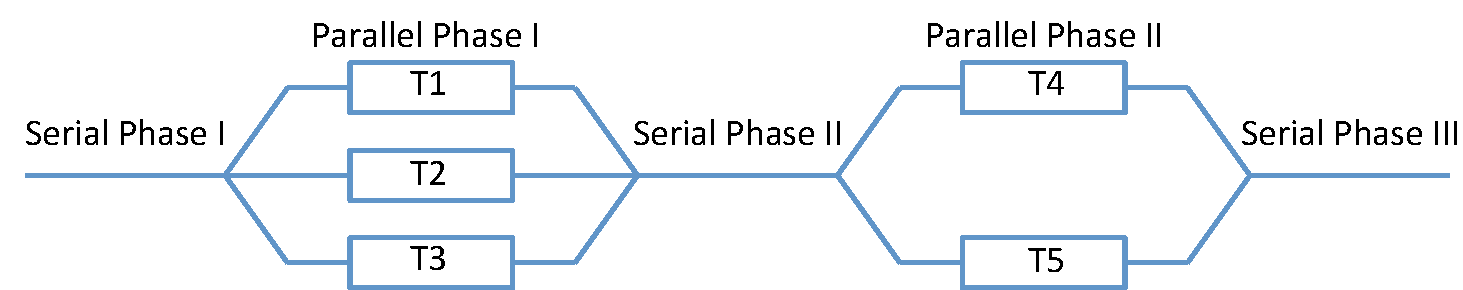
\includegraphics[width=6.5in]{figure/forkjoin}
\end{center}
\caption{\Cheetah{} assesses the impact of false sharing instances of applications with the fork-join model.
\label{fig:forkjoinmodel}}
\end{figure*}

\cheetah{} predicts the impact of an falsely-shared object $O$ on the application into three steps as follows. 

\begin{itemize}
\item \cheetah{} first evaluates how much , which is discussed in Section~\ref{object}. 
\item Then we discuss on the 
\item
\end{itemize}


%Why? The execution of different threads? Performance are closely related to a lot of events, such as cache uses, scheduling, thread-core affinity, locality. Our attempts is just the first try to give some upper bound.  For example, ~\cite{qinzhao} paper. 

But we will try to resolve this and evaluate the precision of our assessment in Section~\ref{}. 

Since we already know this situation, \cheetah{} currently focuses on the widely used and most important execution model -- fork-join model. All applications evelauted .. 


To assess 

These two questions are actually hard to answer, without knowing the running situations of different threads. 





\subsection{Impact on Accesses of this Object}

\subsection{Impact on Related Threads}

\subsection{Impact on the Application}

\subsection{Basic Idea}

\cheetah{}'s assessment is based on the following observations:

\begin{itemize}
\item we can use the results of sampling to represent the whole execution because sampling is evenly distributed over the whole execution. Based on the similar observation, exiting work like Oprofile and Gprof uses the sampling technique to identify the hotspots of function calls and code~\cite{oprofile, DBLP:conf/sigplan/GrahamKM82}.

\item PMU hardware provides the latency information (e.g. cycles) of each memory load operation. We also observed that the latency of accessing falsely shared objects is significantly higher than that of normal accesses. 

\end{itemize}

Based on these two observations, {\bf we propose to use the sampled cycles of an execution to represent the execution time or the runtime}. \cheetah{} will compute the performance improvement based on EQ.(\ref{eq:improvement}), where runtime is denoted by $RT$.
\begin{equation}
\label{eq:improvement}
Perf_{improve}=RT_{actual}/RT_{predict}
\end{equation}


%Thus, based on this equation, the most important thing is to compute $RT_{predict}$, which can be represented by the cycles of accesses after fixing a false sharing instance. $RT_{actual}$ can represented by the sampled cycles of accesses.

%Although it is impossible to know the exact cycles after fixing a false sharing instance, we can estimate based on our two observations as follows. 

To assess the performance impact of a falsely-shared object $O$, \cheetah{} has to collect the following information. 
 
\begin{itemize}
\item $Cycles\_O$: total cycles on a falsely-shared object $O$.
\item $Accesses\_O$: total number of accesses on the object $O$.  
\item $AverageCycles\_{nofs}$: the average cycles of every memory access on non-falsely-shared (abbreviated as ``non-FS'') objects. \cheetah{} utilizes the average cycles of each access that happened in the serial phases as the $AverageCycles\_{nofs}$. There is no false sharing problem in serial phases since there is only one thread in total.  

\end{itemize}

Based on EQ.(\ref{eq:improvement}), we compute the potential performance improvement as EQ.(\ref{eq:improvement2}). Here, we utilize $Cycles\_O$ to represent $RT_{actual}$, while  $RT_{predict}$ can be represented by the product of $Accesses\_O$ and $AverageCycles\_{nofs}$. For $RT_{predict}$ , we assume that the number of accesses after fixing keeps the same (e.g. $Accesses\_O$), and the best latency of each access after fixing the false sharing problem of the object $O$ will be equal to $AverageCycles\_{nofs}$. {\bf This is the basic idea of \cheetah{}'s assessment}. 

\begin{equation}
\label{eq:improvement2}
 Perf_{improve}= Cycles\_O/(AverageCycles\_{nofs} * Accesses\_O);
\end{equation} 



% Now we are going to discuss how to utilize this idea to actually compute the performance of multithreaded programs.  

% How to predict the runtime after fixing false sharing. We are 
% using the cycles of non-fs objects and fs-objects. 
% the number of accesses, and the total number of cycles of fs objects. 

The EQ.(\ref{eq:improvement2}) tells the performance improvement of accesses on a false sharing object. But our final target is know the improvement of the  application itself by fixing a false sharing instance inside. To achieve the final target, we have to compute the following two more things:

\begin{itemize}
\item How much performance improvement each involved thread can get by fixing this instance?

\item How much performance improvement the total application can get by fixing this instance? 

\end{itemize}

These two questions are actually hard to answer, without knowing the running situations of different threads. For example, if a thread is not in the critical path of the performance, then fixing false sharing problems in this thread will not have an explicit impact on the final performance. The assessment can become even more complicated if there are some nested threads in the application. 

To approve the basic concept, 
%\cheetah{} collects the execution information on different phases, different threads, and different objects. 

This section will present the details of \cheetah{}'s prediction. We first describe the general idea using the Figure~\ref{fig:forkjoinmodel} as an example. In this example, only thread $T1$ and $T2$ are involved in a falsely-shared object $O$, \cheetah{} has to know the following information:

 

\subsection{Collecting Execution Information}
\label{sec:getactualtime}

\paragraph{Threads Model Information:} For fork-join models, only the main/initial thread can perform spawning operations. It is easy to verify this by intercepting spawning functions, such as the \texttt{pthread\_create} functions of programs using the \texttt{pthreads} library. 

\paragraph{Phase information:} \Cheetah{} collects the execution time of different serial and parallel phases using RDTSC (ReaD-Time Stamp Counter) on X86 machines.  The difference between the stopping point and the starting point will be considered as the length of a phase. It is relatively easy for \cheetah{} to collect the length of serial phases since \cheetah{} intercepts the spawning operations. For the same reason, \cheetah{} gets the timestamps of the starting point and the stopping point of each thread, then uses the longest span of each thread as the length of every parallel phase. \Cheetah{} also tracks the number of accesses and the cycles of every accesses in serial phases. It uses the average cycles of every memory access in serial phases to be the $Cycles\_{nofs}$ discussed above.  
 
\paragraph{Threads Information:} \Cheetah{} collects the following information of different threads: execution time, number of accesses, and number of cycles of all memory accesses. 

\paragraph{Objects Information:}
For each cache line, \cheetah{} gathers the number of cycles on each cache line. \cheetah{} also collect the number of accesses on each word. Thus, we can compute the number of cycles and accesses on falsely-shared objects. 
 
\subsection{Predicting Execution Time after Fixes}
\label{sec:predicttime}

\cheetah{} predicts the execution time after fixes by replacing the actual cycles of every memory access on a falsely-shared object with the average cycles of a memory access without false sharing. 

According to this, \cheetah{} should know the average cycles of a memory access without false sharing and true sharing. \Cheetah{} actually utilizes the cycles of every memory access in serial phases (denoted as $Cycles_{nofs}$) to approximate this value, which is reasonable since all memory accesses in serial phases should not involve in both false sharing and true sharing. 

Actual cycles of every memory access that are involving in a falsely-shared object can be changed from one execution to another. Thus, \cheetah{} utilizes the total number of all memory accesses instead to predict the performance impact. \Cheetah{} computes the possible performance improvement prediction in the following steps.
 
\begin{enumerate}
\item \cheetah{} first compute the total number of accesses ($Accesses_{fs}$) on suspected cache lines and the total cycles of accesses ($Cycles_{fs}$) on suspected cache lines.

\item For threads that are involved a particular false sharing, \cheetah{} then compute the total number of accesses ($Accesses_{threads}$) and the total cycle of accesses ($Cycles_{threads}$). 

\item \Cheetah{} computes the estimated cycles of those threads that are involved in false sharing according to the formula $Cycles_{pred} = Cycles_{threads} - Cycles_{fs} + Accesses_{fs} * AverageCycles_{nofs}$. 

\item  Based on this, \cheetah{} will compute the performance improvement on threads that are involved in false sharing.
$RT_{threads} = Cycles_{threads}  $. 

\end{enumerate}



\cheetah{} will utilize the latency information of every access to predict the performance impact of a certain false sharing instance. These latency information, normally CPU cycles of every sampled memory access, can be provided by hardware PMUs. \Cheetah{} plans to track detailed memory accesses on falsely-shared objects and on normal objects without false sharing. Thus, we can know the average cycles of every memory access without false sharing. 

\cheetah{} provides a upper bound on performance improvement after fixes. 

It is note that sampling based approaches can actually 
.

We only compute the cycles and threads for the parallel phases. 

\subsection{Predicting Performance Improvement}

Using the $ImproveRate$, we can compute the possible runtime of $T1$ and $T2$ after fixing the false sharing problem of object $O$, which are equal to the product of the actual runtime and $ImproveRate$. If the computed runtime is less than the length of $T3$ in parallel phase I, fixing the false sharing problem of object $O$ won't contribute any performance improvement of the program. Otherwise, it can benefit the performance. Then we compute the new runtime of parallel phase I, which equals to the longest runtime of thread $T1$, $T2$ or $T3$. Based on this, we computes the new runtime of this program, where the execution time of other phases should not be affected. In the end, \cheetah{} predicts the possible performance rate of fixing every false sharing problem so that programs can focus on those important problems.
%There are several steps to evaluate the performance impact. We will consider the average cycles on every access in serial phases as $Cycles_{serial}$. 

 % How to avoid huge performance overhead? We introducing per-thread recording mechanism. 

% How to actually predict the performance improvement? A thread may have the serial part and parallel part. We have to identify the serial part and parallel part. 

% How to handle different CPUs? For example, we may start 16 threads on 8 CPUs. 

% Can we get the resolute time on each phase? We are using this to calculate the performance improvement.  We also copy the whole memory accesses information out before transferring phases. 

% What if only two threads only accesses a specific cache line and other threads didn't accesses that? We can actually check the word level's accesses to find out those number of threads that are accesses this tid. We could also verify whether those memory accesses are on the critical path or not. 

% We should use actual tid instead of thread index to identify threads. 

% We should remove the write-invoked tracking since we have to check the number of accesses. Thus, we actually don't care those ones that are happened in the serial phase. Because we won't actual change its performance initially. 



% The total number of memory accesses on an addresses

% The total latency of accessing an address

% The total number of memory accesses for each thread. 

% The total latency of all memory accesses for each thread  

% All memory accesses of each thread

% All memory accesses in total = Sum of (memory accesses of each thread)

% Total latency of all memory accesses for each thread. 